\documentclass{article}
\usepackage{style}

% Additional packages
\usepackage{subfig,float}
%\captionsetup[subfloat]{farskip=-1mm,captionskip=-1mm}
\newcommand{\twa}{0.45\textwidth}
\newcommand{\twb}{0.3333333333\textwidth}
\usepackage{tabularx}
%\newcolumntype{C}[1]{>{\centering\arraybackslash$}p{#1}<{$}}
\setlength{\arrayrulewidth}{1.0pt}

% Define colors
\usepackage{color}
\definecolor{orange}{rgb}{1,0.5,0}
\definecolor{amethyst}{rgb}{0.6,0.4,0.8}
\definecolor{aureolin}{rgb}{0.99,0.93,0.0}
\definecolor{awesome}{rgb}{1.0,0.13,0.32}
\definecolor{ao-green}{rgb}{0.0, 0.5, 0.0}
\definecolor{MSBlue}{rgb}{.204,.353,.541}

% Define commands for communication between us
\newcommand{\ferran}[1]{\textcolor{green}{#1}}
\newcommand{\javier}[1]{\textcolor{blue}{#1}}
\newcommand{\lluis}[1]{\textcolor{orange}{#1}}
\newcommand{\chat}[1]{\textcolor{amethyst}{#1}}
\newcommand{\review}[1]{\textcolor{red}{#1}}

%commands to manage sections, figures and acronyms
\usepackage{doi}
%\usepackage{tikz}
%\usetikzlibrary {positioning,intersections,fit,shapes.geometric}
%\newcommand{\fig}[1]{Figure~\ref{fig:#1}}
%\newcommand{\sect}[1]{Section~\ref{sec:#1}}
\usepackage{acronym}
\acrodef{hpc}[HPC]{high performance computing}
\acrodef{cpu}[CPU]{central process unit}
\acrodef{gpu}[GPU]{graphics processing unit}
\acrodef{dns}[DNS]{direct numerical simulation}
\acrodef{mhd}[MHD]{magneto-hydro-dinamics}
\acrodef{upo}[UPO]{unstable periodic orbit}
\acrodef{pod}[POD]{proper orthogonal decomposition}
\acrodef{dmd}[DMD]{dynamic mode decomposition}
\acrodef{sindy}[SINDy]{sparse identification of nonlinear dynamical systems}
\acrodef{bvae}[$\beta$-VAE]{beta-variational autoencoders}
\acrodef{res}[RES]{Red Española de Supercomputación}
\acrodef{prace}[PRACE]{Partnership for Advanced Computing in Europe}
\acrodef{bsc}[BSC]{Barcelona Supercomputing Center}
\acrodef{upc}[UPC]{Universitat Polit\`ecnica de Catalunya $\cdot$ BarcelonaTech}


\usepackage{pgfplots}
\usepackage{graphicx}
\usepackage{fancyhdr}
\pagestyle{fancy}
%\usepackage{xcolor}
\usepackage[dvipsnames]{xcolor}
\usepackage{lipsum}
\setlength\headheight{26pt} %%
\usepackage{hyperref}
\usepackage[final]{pdfpages}
\usepackage{stix}
\usepackage{float}
\usepackage{caption}
\usepackage{tabularx}
\usetikzlibrary {arrows.meta} 
\usetikzlibrary{decorations.markings}
\usepgfplotslibrary{colormaps}
%\usepackage[titles]{tocloft}
\usepackage{enumitem}
\usepackage{multirow}

%\setlength{\cftbeforechapskip}{50pt}
%\pgfplotsset{width=7cm,compat=newest,axis line style={draw=none},ticks=none}

%\lhead{\includegraphics[width=0.2\textwidth]{nyush-logo.pdf}}

%\fancypagestyle{firstpage}{%
%  \rhead{\Large HAP-Calafell}
%  \lhead{
\includegraphics[width=5cm]{logo-upc}}
%}

\fancypagestyle{firststyle}
{
   \fancyhf{}
   \fancyhead[L]{
\includegraphics[width=5cm]{logo-upc}}
   \fancyhead[R]{\Large PT-Calafell}
}

\pagestyle{fancy}
\fancyhf{}
\fancyhead[L]{
\includegraphics[width=5cm]{logo-upc}}
\fancyhead[R]{\Large PT-Calafell}
\fancyfoot[R]{Page \thepage}

%%%% PROJECT TITLE
\title{{\bf Pla de Treball / Work Plan}}
\date{}
\author{\Large Joan Calafell Sandiumenge}

\begin{document}

\maketitle


\thispagestyle{firststyle}

\vspace{1.0cm}

\begin{tabular}{ l l }
\hline \\
 Site Code:          & 71025761-71025762  \\ 
 Position Reference: & LE-27-28/729 \\
 Unit of assignment: & 729- Fluid Mechanics Department  \\  
 Field of Knowledge: & Industrial Engineering \\
 Area of Knowledge:  & Fluid Mechanics \\   
 Linked Unit:        & Escola d’Enginyeria Barcelona Est (EEBE)\\
  $\ $               & $\quad $$\quad $$\quad $$\quad $$\quad $$\quad $$\quad $$\quad $$\quad $$\quad $$\quad $$\quad $$\quad $$\quad $$\quad $$\quad $$\quad $$\quad $$\quad $$\quad $$\quad $$\quad $$\quad $$\quad $$\quad $$\quad $$\quad $$\quad $$\quad $$\quad $$\quad $$\quad $$\quad $$\quad $$\quad $$\quad $$\quad $$\quad $\\
 \hline
\end{tabular}

\newpage

\tableofcontents

\newpage

\section*{Personal Data}

\vspace{0.5cm}

\begin{tabular}{ l l }
 {\bf Name:}               & Joan Calafell Sandiumenge  \\ 
 {\bf ID Number:}          & 44019853S \\
 {\bf Nationality:}        & Spanish  \\  
 {\bf Date of Birth:}      & 14/06/1978 \\
 {\bf Address:}            & Guifré 8 3er 1a 08001 Barcelona \\   
 {\bf Phone:}              & +34 669 14 36 49\\
 {\bf E-mail:}             & joan.calafell@upc.edu\\
\end{tabular}

\vspace{0.5cm}

\section{Research Plan} 

\subsection{Research Background} 

In 2012 I started my first research line from scratch, focused on new wall modeling approaches for Large Eddy Simulations (WMLES) to enable high-Reynolds number aerodynamic simulations of industrial-relevant applications. Since then, I kept working in this research line which has been my primary research topic so far \cite{CAL19,ALJ18}. I have investigated from relatively simple equilibrium wall functions to complex non-equilibrium Two-Layer and data-driven models. 

Due to my background in computational aerodynamics, in November 2019, I joined the Large-Scale Computational Fluid Dynamics Group (LSCFD) of the Barcelona Supercomputing Center  \href{https://www.bsc.es/discover-bsc/organisation/research-departments/large-scale-computational-fluid-dynamics}{(see LSCFD website)}. In that position, I opened the environmental flows research line. The initial purpose was to apply my knowledge of WMLES to urban flow and high-resolution pollutant dispersion prediction.
Due to the surge of Deep Learning (DL) and its massive potential for CFD modeling development \cite{KUT17}, in October 2020, I enrolled a postgraduate program in Deep Learning at the UPC to learn the fundamentals of the most advanced techniques in the area. This allowed me to apply these techniques to my two primary research lines while acquiring a horizontal role within the LSCFD group by promoting AI-based methods in various research lines of the group. Currently, I am involved in the following specific research areas:

\begin{itemize}

\item Data-Driven wall modeling for high-Reynolds number aerodynamics:

This research line focuses on developing wall modeling strategies based on different AI approaches to allow large high-Reynolds and high-Mach number aerodynamic simulations for applications such as aeronautics, environmental flows, automotive, and turbomachinery. Specifically, an XGBoost-based model trained with wall-resolved LES data from a 3D Diffuser has been developed. The model has been able to predict laminar to turbulent transition, a breakthrough in wall modeling. On the other hand, I am also working on applying state-of-the-art Graph Neural Network architectures for wall modeling with the purpose of enhancing WMLES predictive capabilities in complex flow conditions such as those found in urban flows and external aerodynamics.  
%{\color{red} comentar d'alguna manera que el wall modeling s'està aplicant al nextsim}


\item Computational and data-driven urban flow and pollutant transport predictive models: 

This research line is being tackled through both computational and data-driven strategies. Regarding the computational approach, the research is focused on using high-fidelity WMLES models for urban flow and pollutant transport prediction in urban environments. Most works published in this area are performed with Reynolds-Averged Navier-Stokes (RANS) modeling. The development of numerical frameworks for WMLES urban flow simulations is a state-of-the-art topic \cite{TOP17}. 

The data-driven strategy is intended to enable high-resolution wind flow \cite{MOK21,HOI22} and pollutant concentration fast prediction, which is unfeasible by using computational techniques. The models rely on deep convolutional neural networks (NN), which generate high-resolution wind flow and pollutant concentration maps using urban geometry, pollutant emission sources, and meteorological data as input. A vast dataset relating the input/output data has been generated through WMLES simulations to allow supervised NN training. 

The methodology has been developed in different applied competitive projects in which predicting capabilities are being successively added. At present, the research line is evolving on two fronts, generalizing the neural network architectures to allow 3D predictions and extending the existing dataset with porous media-based simulations to allow capturing vegetative canopy effects.

Also, within this research area, I am also working on enhanced passive scalar transport modeling methods. The idea is overcoming the limitations of the Gradient Diffusion Hypothesis when dealing with the time-averaged passive-scalar transport equations. A set of correlations is being created to evaluate the scalar flux magnitude from flow-relevant quantities. The challenge is solved as a non-linear regression problem implemented through a Multilayer Perceptron Neural Network and trained with high-resolution data of a wall-mounted cube case with passive scalar transport phenomena (CEDVAL A5 experiment). The purpose is to improve pollutant dispersion modeling in momentum-coupled and convection-diffusion problems. 

In parallel, I am also working on data-driven models for turbulent flow analysis. Specifically, I am investigating state-of-the-art Variational Autoencoder (VAE) architectures for non-linear modal decomposition and flow reconstruction. The ultimate purpose is to gain fundamental insight into the flow physics of bluff bodies and other wall-bounded flows, such as urban flows, to develop reduced-order models and methodologies to support my primary research lines commented above. At present, I am directing a Bachelor Thesis on this subject (see HAP document) whose defense will be on 18th July 2023.

\end{itemize}


\subsection{Research Ojectives}  \label{sec:res-obj}

The European Green Deal, approved in 2020, is a set of policy initiatives of the European Commission with the overarching aim of making the European Union (EU) climate neutral by 2050 \href{https://www.euractiv.com/section/energy-environment/news/eu-commission-unveils-european-green-deal-the-key-points/}{(see link)}. The objectives outlined in this research plan are aimed at helping to meet these objectives.    

The proposed research lines will build on my previous research and focus on computational and data-driven techniques for both wall modeling and environmental flow prediction. The objective is to contribute to the EU's targets by allowing aerodynamic efficiency improvement to reduce energy consumption and, second, minimize the impact of pollutant technologies on public health and the environment during the transitional period and beyond.

Within these two main applied research lines, I will work on some fundamental problems with the purpose of creating the necessary tools to successfully advance the main objectives. 

On the other hand, I plan to develop the proposed research lines by creating as many synergies as possible with UPC researchers. I am entirely open to adapting them to mutually complement our research lines and boost the research group's performance from a quantitative and a qualitative point of view. 

In the following sections, a detailed description of my research proposals and objectives is given. Then, the resource procurement strategy will be explained, and finally, a detailed work plan to successfully complete the objectives will be outlined. 

\subsubsection{Data-Driven Wall Models for high-Reynolds and high-Mach number aerodynamics}

Among the 2030 Grand Challenges identified by NASA, the LES of a powered aircraft configuration across the entire flight envelope appears in the first position of the priority list \cite{SLO14}. In NASA's report, Wall-Modeled LES (WMLES) is proposed as the primary strategy to circumvent the massive costs of accurately resolving the boundary layer while benefiting from the temporal and spatial resolution of an LES computation. 

Existing wall modeling approaches have traditionally been based on establishing a relation between the resolved outer layer and shear stresses at the wall through physical models. Those models account for the non-resolved inner layer flow feature effects, crucial in the actual wall shear stress formation. However, most models are derived through strong physical assumptions, significantly reducing their generality \cite{BOS18}. Moreover, traditional wall modeling strategies only take small amounts of data from the LES-resolved outer layer. This data feeds the physical model that ultimately produces a shear stress value. 

In recent years, the wall modeling community has witnessed a significant surge in the use of data-driven techniques  \cite{VAR23} intended to circumvent the limitations of traditional models. The proposed strategies have been based on establishing a non-linear linking function between the input data and the expected output. This allows for getting rid of external and not general physical models. 

Most models proposed use shallow multilayer perceptron (MLP) architectures \cite{VAR23} to create the non-linear function. The use of MLPs implies vast amounts of trainable parameters, even for small networks. This hampers the use of large input data samples and the application of deep neural networks (DNN), preventing the model from exploiting DNN's capability of "understanding"  complex relations as those found in a near-wall flow on their own. 

To overcome these limitations, I plan to use Graph Neural Networks (GNN) for wall modeling applications. I presented preliminary work on this subject at the IUTAM conference in Aarhus, Denmark, in 2022. GNNs are especially suited for computational fluid dynamic (CFD) problems since data is arranged in either spatially structured or unstructured meshes, which are particular cases of graphs \cite{ZHO20}. On the other hand, the GNN computational efficiency would allow large input data batches \cite{GAO22}, allowing the model to have a large physical context of the outer layer physics and, thus, taking into account long-range effects such as adverse pressure gradients. Additionally, this would allow deeper neural networks permitting the GNN to extract the complex underlying physics while keeping a reasonable network size. These characteristics are expected to significantly increase the model's predictive capabilities in complex flow configurations. Moreover, this will impact two crucial aspects, the network training cost and, even more important, the reduction of the inference time during the simulation. 

As a practical application, I plan to use the developed methodologies for active flow control analysis. Some relevant works on state-of-the-art flow control methodologies powered by Machine-Learning methods \cite{GUA23} have been recently published. The proposed flow control strategies are based on placing actuators on solid surfaces in contact with critical boundary layer regions. These actuators are numerically modeled through boundary-normal mass flow injections. An innovative flow control approach proposed by Rabault et al. \cite{RAB19} uses multi-agent reinforcement learning to control the mass injection frequency and intensity to minimize the total aerodynamic drag. My idea is to evaluate the performance of these innovative devices through high-fidelity WMLES simulations.

\subsubsection{Data-driven high-fidelity fast predictive models for environmental flows}

This research area builds on my current work at the Barcelona Supercomputing Center on fast high-resolution predicting tools for Urban flow and Pollutant dispersion. Existing NN-based models only consider solid building geometry and meteorological conditions to predict wind flow and dispersion patterns. However, urban areas are affected by other phenomena, such as vegetative canopies, small obstacles, and atmospheric thermal effects, which strongly influence the wind and pollutant dispersion mechanisms. 

This research line is intended to successfully add physical background to current models in order to increase their range of applicability and accuracy. I have an active project in which I am creating an extensive dataset by means WMLES that will allow the introduction of the vegetative canopy effects on the neural network predictions. The urban vegetative regions are modeled through a porous media sink term in the momentum equation \cite{VIA21}. Later, the canopy's geometrical and density characteristics will be appropriately encoded to provide relevant physical input to the NN.

Furthermore, the current methodology relies on the fact that urban-like flow patterns become Reynolds number-independent for sufficiently large $Re$ values \cite{LIM09}. This property is leveraged to significantly reduce the training dataset size by assuming a constant geostrophic pressure gradient magnitude for the whole dataset. Then, the NN output is scaled to meet the actual meteorological conditions. Unfortunately, Reynolds number independence is not fulfilled when thermal buoyancy effects are considered. Thus, adding thermal effects in the flow predictive NN would entail the generation of a disproportionate dataset to account for a reasonable number of geostrophic pressure gradients and thermal condition combinations. 

To overcome this bottleneck, I want to investigate the development of a NN that runs on top of the existing wind flow predictive model. This new NN would introduce thermal-induced effects such as vertical convection by correcting the original wind field a posteriori. To train the corrective NN, a dataset linking geostrophic pressure-driven flows with their equivalent flow with thermal effects would be created. Uncoupling the pressure-driven and thermal effects should make the dataset generation feasible.

Moreover, urban areas are filled with obstacles at the pedestrian level, such as parked car rows or trash bins, which can also distort the dispersion patterns. Unfortunately, most of these obstacles lay within the inner boundary layer, which is not explicitly resolved in WMLES, and thus, they cannot be represented in the existing high-fidelity datasets. Explicitly resolving the inner layer for extensive urban areas is at present unaffordable. I propose using a posteriori neural network that introduces flow corrections downstream of the obstacles to approximate their effects. This approach assumes locality and the effects far downstream will be neglected. The accuracy of this assumption will be assessed. 

On the other hand, current approaches provide time-averaged patterns for wind and pollutant dispersion predictions. One of the open fronts in this research area is to introduce temporal predictive capabilities through data-driven reduced-order modeling (ROM). At present, I already started to lay the foundations of this strategy by investigating turbulent flow nonlinear modal decomposition through Variational Autoencoder Neural Network architectures. Below, the global strategy to reach this goal is outlined: 

The chaotic and multiscale nature of turbulent flows makes it significantly difficult to understand their physical behavior. This makes the creation of reliable predictive methodologies complex. However, turbulent flows show recognizable spatial and temporal patterns that might be unveiled through existing methodologies, shedding light on this complex physical phenomenon. Traditional techniques have been based on linear projection techniques such as proper orthogonal decomposition (POD) or dynamic mode decomposition (DMD) \cite{EIX22}, which decompose turbulent flow phenomena into different classes of energetic modes. However, the linear nature of these methodologies limits their ability to capture relevant flow characteristics. 

Recent works have shown the ability of beta-Variational Autoencoders ($\beta$-VAE) to extract nonlinear modes from turbulent flow \cite{EIV22}, which may help overcome the linear model limitations. $\beta$-VAE methods are based on probabilistic neural networks (NN) that can extract minimal and near-orthogonal sets of nonlinear modes from high-fidelity turbulent flow data. One of the method's main advantages is that notable flow reconstruction accuracies are obtained with a significantly small number of modes compared to linear approaches. Nevertheless, current implementations rely on 2D architectures, which collide with the 3D nature of turbulent flows. Moreover, another significant limitation of $\beta$-VAEs is their need to work with regular image-like grids. This is because $\beta$-VAE's architecture primarily comprises convolutional neural networks (CNN) that have been developed to work on images rather than flow simulations. However, there is no theoretical restriction on working with spatially unstructured data. To overcome these two major restrictions, I plan to investigate the use of Graph Neural Network architectures to allow 3D unstructured data processing through $\beta$-VAE's.

In parallel, long-term flow prediction based on $\beta$-VAE's will be explored. The proposed strategy leverages the encoding ability of $\beta$-VAE of turbulent flow to create ROMs for long-term flow prediction. Data-driven ROMs for turbulent flow prediction is a flourishing research field with many different strategies recently proposed, e.g., \cite{LEE21,LOP21,ABA22}. The general conclusion of these works is that using specific time series architectures, namely recurrent neural networks (RNN), significantly increases the long-term predictive capability of the models. However, unlike convolutional neural networks (CNNs), which are designed for image processing, RNNs are developed for data sequence processing and are thus unsuitable for large data samples. To circumvent this limitation, all authors using RNNs resort to POD to reduce the dimensionality of the training database. As a result, the DNN is only required to predict the time series of the scalar temporal coefficients for each temporally-independent POD spatial mode \cite{ABA22}.

Here is where $\beta$-VAEs come in. My proposal is leveraging the low dimensionality of $\beta$-VAE's latent space vector to predict the temporal evolution of its components. Then,  the flow field would be recovered by decoding the predicted latent space. Given the nonlinear nature of the model, it is expected that this approach will be a more suitable approach for turbulent flows than existing linear POD-based models. Moreover, given the small size of $\beta$-VAEs latent space vectors [${\cal O}(5)$] compared to the necessary number of POD temporal modes for 3D flow reconstruction [${\cal O}(10^2)$], the number of coefficients to be predicted will be drastically reduced. It is expected that these properties will lead to a significant improvement in the model's predictive capabilities and efficiency.

Another crucial aspect of this research line is dataset generation for training purposes. However, this can be extremely expensive if high-fidelity models are used to create data. In the context of my current research projects, a vast dataset for pollutant dispersion fast prediction has been created. This dataset comprises 450 high-resolution pollutant emission scenario simulations for 90 different meteorological conditions in 30 different urban geometries. The wind flow configurations were simulated through WMLES in urban geometries covering 1x1 km areas at 1-meter resolution, requiring meshes of more than 100 million elements. In order to allow the 450 pollutant dispersion simulations, the emission scenarios were modeled as a convection-diffusion problem in which the time-averaged WMLES fields were used as a transport field. 

Nevertheless, the prediction quality of time-averaged passive-scalar transport equations depends on the accuracy of the underlying models and hypothesis introduced to model the unclosed scalar flux term. This term appears when averaging the instantaneous passive-scalar transport equation. The simplest model to approximate the scalar flux term is the so-called Gradient-Diffusion Hypothesis (GDH), which assumes that the scalar flux is proportional to the gradient of the mean scalar magnitude. The proportionality constant is the turbulent diffusivity, defined as the ratio of the turbulent viscosity and the Schmidt Number in the case of a substance transport. However, it has been reported in homogeneous shear flows that the errors for GDH models are not negligible \cite{TAV81}. In particular, the implicit assumption in GDH that the scalar flux and the mean scalar gradient are aligned is invalid in near-wall regions, widely present in urban flows and many other applications of interest \cite{WEA20}. Another source of error is the constant Schmidt number assumption which is questionable in many flow conditions \cite{WEA20}. 

The proposed strategy to improve the modeling techniques builds on previous works of several authors \cite{MIL18,WEA20}. It is based on replacing the traditional but physically-limited gradient-diffusion hypothesis with a non-linear data-driven model that takes more physical context from the time-averaged solution. The concept assumes that the scalar flux depends not only on the Reynolds stress and the passive scalar concentration gradient but also on other Galilean invariant quantities, such as the strain and rotation rate tensors. Then, a function linking these flow quantities with the unclosed scalar flux is determined. However, all the proposed works use limited regression methodologies, such as Random Forests or Gene Expression Programming to determine the linking function. In that sense, I plan to improve the methodology by using advanced nonlinear models based on Multilayer Perceptrons to create the expression relating the flow magnitudes with the scalar flux term. To do so, a dataset based on canonical flows, namely, a wall-mounted cube representing the characteristic physics of urban flows, will be created to enhance the model capabilities for these specific conditions.

A fundamental aspect of computational and data-driven modeling is the availability of experimental data for validation. This aspect has been considered in my current research projects in which field reference data has been collected. Nevertheless, the meteorological and pollutant sensor networks deployed during the projects are relatively small due to budget limitations. In that sense, I plan to explore recent advances in machine learning and data assimilation \cite{ALM22,ARC21} to enhance measured data quality, following recent works which used these methodologies for Particle Image Velocimetry (PIV) \cite{HAS23} or Particle Tracking Velocimetry (PTV) \cite{MON22} measurement enhancement. Moreover, some physical quantities, such as wall shear stress or spatial density variations, may be extremely difficult to measure. In this regard, the proposed methodologies are also suitable to infer derived flow variables (pressure, wall shear stress, or fluid density, among others) from measured primitive variables.

Finally, a relevant factor in improving the deep-learning-based methods intended to model physical phenomena is the enforcement of physical and/or thermodynamic constraints in the model through the loss function to ensure physical laws fulfillment, i.e., mass, momentum, or energy conservation, among  others \cite{LEE21}. This strategy, also known as constrained or physics-informed neural networks  (PINNs) \cite{RAI17}, will be systematically applied whenever possible.


\subsubsection{High-Performance Computing Strategy}

High-Performance Computing (HPC) is a fundamental working tool in my research \cite{VOL19}. It is essential for all the research phases, from computational and data-driven model development to dataset generation. 

In that sense, I have worked with many HPC architectures: Intel-based clusters (MareNostrum 3, MareNostrum4, Picasso, AMD-CTE, JFF) and, more recently, GPU-based clusters (CTE-Power). Thus, I have always worked with state-of-the-art competitive clusters using the latest HPC technologies. I have also developed a wide variety of efficient and massively parallel applications, primarily written in C++ for flow solvers and Python language for data postprocessing and deep learning training. These codes have been efficiently executed on the supercomputers mentioned above. 

As with any programming language, both C++ and Python have strengths and weaknesses. C++ is the default language of Scientific Computing. It is mature, computationally efficient, has a vast ecosystem, and most modern heterogeneous compute environments (Cuda/Sycl, etc.) are developed for C++. Moreover, its object-oriented nature allows the development of modular and clean codes. However, C++ lacks specific libraries for machine learning model development, making it necessary to resort to external interfaces to link data-driven models. 

By contrast, Python has a wide variety of data science and machine learning ready-to-use packages (Pytorch, TensorFlow, Keras, Scikit-learn, among others), making Python one of the most widely used high-productivity languages in Scientific Computing. Unfortunately, the language does not natively support the type of data structures and other features needed for fast computations, and its memory management tools are minimal, hampering the use of Python for HPC purposes.

In that sense, Julia is a relatively recent programming language that has quickly built up a sizeable support community. Even though Julia is a high-level language, it has been successfully used for simulations at Petaflops scale. Moreover, it also features machine learning libraries for data-driven model development which can be straightforwardly integrated with the computational simulations. On top of that, JuliaGPU provides packages for GPU programming, a critical requirement considering current HPC hardware trends. As an illustrative example, around 80\% of the MareNostrum V supercomputer will be composed of NVIDIA H100 Tensor Core GPUs.  
Considering these advantages, using Julia language for computational and data-driven modeling is part of my research strategy.


\subsection{Resource Procurement} \label{sec:resources}

Procuring financial and computational resources is an essential part of the integral strategy to realistically achieve the proposed research objectives. These resources will make possible Ph.D. student and postdoc researchers' hiring, license and equipment purchase, and obtain the necessary computational resources to perform extensive numerical simulations and training data-driven models. In that sense, I have broad experience writing competitive project proposals with a significant success rate (see HAP document). Regarding the competitive computing allocation projects, I have been the Principal Investigator of 5 projects. 

\subsubsection{Financial Resources}

Financial resources will be obtained through competitive European, National, and Autonomic funding projects. These projects will be written as Principal Investigator whenever possible. Regarding fundamental research calls, I plan to submit individual and shared proposals with other research group members and external collaborators. For applied research calls, consortiums will be promoted with leading companies and research centers, leveraging the extensive network of contacts I made in my current and past positions. Below, a list of potential competitive calls to apply based on open or recently closed programs is shown. In the case of expired programs, I will apply to equivalent future calls:

{\bf Fundamental Research:}

\begin{itemize}[noitemsep]
\item Agencia Estatal de Investigación: 
\begin{itemize}[noitemsep]
\item[·] Generación de Conocimiento
\item[·] Redes de Investigación
\end{itemize}
\end{itemize}


{\bf Applied Research:}

\begin{itemize}[noitemsep]
\item European Commission: 
\begin{itemize}[noitemsep]
\item[·] EuroHPC Joint Undertaking.
\item[·] Horizon Europe.
\item[·] Clean Aviation.
%\item[·] {\color{red} Clean Hydrogen posar a MMT}
\item[·] European Defence Fund.
\item[·] European Space Agency: Innovation Triangle Initiative.
\item[·] Programa INTERREG V-A España-Francia-Andorra (POCTEFA).
\end{itemize}
\item CDTI: 
\begin{itemize}[noitemsep]
\item[·] Misiones Ciencia e Innovación.
\item[·] Programa Tecnológico Aeronáutico (PTA). 
\end{itemize}
\item Agencia Estatal de Investigación: 
\begin{itemize}[noitemsep]
\item[·] Retos-Colaboración publico-privada.
\item[·] Proyectos Estrategicos de Transicion Verde y Digital.
\end{itemize}
\item Generalitat de Catalunya: 
\begin{itemize}[noitemsep]
\item[·] Nuclis d'R+D empresarial, Projectes INNOTEC.
\end{itemize}
\end{itemize}

\subsubsection{Computational Resources}

Computational resources will be obtained through computing allocation competitive calls, namely:

\begin{itemize}[noitemsep]
\item Red Española de Supercomputación (RES)
\item EuroHPC JU
\end{itemize}

On the other hand, upon agreement with my eventual UPC research group, as an ex-BSC researcher, I can establish an official research collaboration with BSC that would grant me unrestricted access to the $10\%$ of BSC computational resources under the same conditions as BSC research staff. Considering the imminent start-up of MareNostrum V with an estimated peak performance of 250 PetaFlops and primarily composed of GPU technology, this will be a significant advantage for me and all my host UPC group members, who could also have access via my account.

\subsubsection{Software tools}

Software tools are essential to develop new physical models for fluid dynamic simulations and to perform the required simulations for flow physics research and dataset generation. Given the general trend in HPC in which CPU-based clusters are being replaced with more computationally efficient GPU architectures, I will prioritize using GPU-supported codes. The codes listed below are open source, or a free license agreement can be obtained for research purposes.

{\bf CFD simulation codes suitable for fundamental research:}

\begin{itemize}
\item {\bf REHA} (Reproducible Hybrid architecture flow solver Engineered for Academia) \cite{JOF23} is available as open-source under the MIT license. RHEA solves the conservation equations of fluid motion for compressible flows on structured meshes through second-order numerical discretizations in combination with kinetic-energy-preserving convection schemes and utilizes explicit Runge-Kutta methods for time integration. The solver is written in C++, using object-oriented programming, utilizes YAML and HDF5 for input/output operations, and targets {\bf hybrid (CPU-GPU)} supercomputing architectures by combining MPI and OpenACC directives.
\end{itemize}

{\bf CFD simulation codes suitable for applied research:}

\begin{itemize}
\item {\bf SOD2D}. This code implements a numerical solution for the equations governing compressible fluid flow in three dimensions. The code is based on the spectral element method (SEM) and designed for scale-resolving simulations (DNS, LES, and WMLES). The code supports unstructured meshes and is then suitable for complex geometries. This code has been developed within the BSC's Large-Scale Computational Fluid Dynamic Group. SOD2D has been developed to efficiently leverage the computational power being deployed worldwide, in which GPU plays a central role. For that reason, it has been developed to be able to {\bf run on either GPU and CPU architectures}. Specifically, the code is written in Fortran, and uses MPI and OpenACC to provide parallelism at both coarse and fine-grained levels. The mesh is partitioned using the GEMPA library, and it uses HDF5 for I/O, which are efficient and widely tested libraries for HPC.

\item {\bf ALYA} Alya is a high-performance computational mechanics code to solve engineering coupled problems \cite{HOU09}. The code is based on the Finite Element method and is suitable for unstructured meshes. The code features low-dissipation FE schemes that allow good accuracy compared to other low-dissipation finite volume and finite difference methods, with the advantage of increasing the order of accuracy at will without breaking the fundamental symmetry properties of the discrete operators. Alya also features wall modeling libraries for the resolution of high-Reynolds wall-bounded flows. {\bf Alya is only suitable for CPU} architectures, a significant drawback regarding its use. 

\item {\bf OpenFOAM} OpenFOAM (for "Open-source Field Operation And Manipulation") is a C++ toolbox for the development of customized numerical solvers and pre-/post-processing utilities for the solution of continuum mechanics problems, including computational fluid dynamics (CFD). OpenFOAM is based on the Finite Volume Method and supports unstructured meshes. Although OpenFOAM runs only on CPU, there are initiatives to port it to GPU \href{https://sim-flow.com/rapid-cfd-gpu/}{(see RapidCFD)}. One of the main strengths of OpenFOAM is its vast user community in areas such as research organizations, academic institutes, and automotive, manufacturing, process engineering, and environmental engineering industries, among others. Thus, contributing to extending OpenFOAM capabilities can have an extraordinary impact on research and industry. 

\end{itemize}

\subsection{Work plan}

This section outlines the work planning to successfully achieve the research objectives. The planned activities in each research line are grouped in work packages, and the temporal sequence is described through a Gantt chart. According to the present call conditions, the offered position is for a temporary contract of six years. Moreover, it must be considered that the Associate Professor Accreditation of the "Agència per a la Qualitat del Sistema Universitari de Catalunya" (AQU) must be obtained before the end of this period. The proposed planning also takes into account that current Ph.D. studies must be completed within three years. Below, the work packages containing the tasks, the required resources, and the expected outcomes are described. Then, in Figure \ref{fig:gantt}, the Gantt chart with the planned timing is shown.

\vspace{0.5cm}

{\bf WP1}
\vspace{4pt}
\hrule
WP1 is intended to secure all the financial, computational, and material resources required to develop the research objectives. This WP will be permanently active since it is essential for the plan development during the six years contract and beyond. The first phase will be devoted to securing the necessary resources to allow the beginning of WP3, WP4, and WP5 on time. The WP activities will be developed according to the resource
procurement strategy outlined in Section \ref{sec:resources}.  \\         {\bf Expected outcome:} Financial and computational resources to execute the proposed research lines.
 \vspace{4pt}
\hrule

\vspace{0.5cm}

{ \bf WP2 }
\vspace{4pt}
\hrule
This work package is devoted to publishing the results obtained in my current research at BSC. At present, I am writing two articles derived from active and finished projects related to urban flow and pollutant dispersion prediction. Moreover, I am also collaborating on writing a paper derived from the research on data-driven wall models with a Ph.D. student whom I advised for the past three years. \\
{\bf Expected outcome:} Three Q1 journal papers.
\vspace{4pt}
\hrule

\vspace{0.5cm}

{ \bf WP3 }
\vspace{4pt}
\hrule

This work package covers the development of the data-driven wall modeling research line. The initial activities are planned to be done in Master's Thesis works. I plan to initiate studies on using Graph Neural networks for 3D spatial unstructured data in this period. Existing datasets will be used, and training resources will be obtained through open-source Google services and RES projects. In case of agreeing on a collaboration with BSC, the MareNostrum V resources would also be available.\\
In the second phase, a Ph.D. work will be conducted with the following objectives: i) creating a GNN-based wall model prototype relating outer flow quantities with wall shear stress in extensive areas; ii) training the model with existing non-equilibrium flow datasets. If required, new data sources will be created; iii) prototype implementation in OpenFOAM;  iv) model validation in canonical flows by comparing with reference results. v) assessment of log-layer mismatch presence and countermeasure implementation. Once the wall model is validated, a Master's thesis will be proposed to analyze active flow control technologies through advanced WMLES.\\
{\bf Required Resources:} For the Ph.D. work, a competitive student grant or fundamental research project funding will be required. Moreover, open-source libraries and codes will be used (Pytorch geometric, Julia, OpenFoam). The computational resources will be obtained through RES projects.  \\
{\bf Expected outcome:} An open-source data-driven wall modeling OpenFoam Library. At least three Q1 journal papers regarding GNN wall model performance, its OpenFOAM implementation, and the WMLES active flow control assessment.
\vspace{4pt}
\hrule

\newpage

{ \bf WP4 }
\vspace{4pt}
\hrule
This work package covers fast data-driven models for high-fidelity environmental flow predictions. Preliminary activities regarding using GNN for 3D unstructured data processing in environmental flows will be done through Master's Thesis works. Existing datasets will be used for this purpose.\\ 
In the second stage, a Ph.D. student will carry out the following tasks: i) creating a posteriori corrective neural network to account for thermal effects; ii) developing a posterior corrective neural network to account for urban small obstacle effects; iii) creating the required training datasets through WMLES with Alya code; iv) scalar flux modeling for time-averaged transport problems. Later, this will be applied to generate a pollutant transport dataset with Alya. v) validating the results with experimental data provided by  Bettair Cities S.L. and other sources.\\
{\bf Required Resources:} For this Ph.D. work, a competitive student grant or an applied research project funding will be required. Moreover, open-source libraries and codes will be used (Pytorch geometric, Julia, Alya). The computational resources will be obtained through RES projects, while existing datasets will be reused.  \\
{\bf Expected outcome:} A high-fidelity and fast tool for urban flow and pollutant dispersion prediction. At least three Q1 journal papers, two related to the thermal and the small obstacle effect corrective neural networks and one to publish the generated datasets. 
\vspace{4pt}
\hrule

\vspace{0.5cm}

{ \bf WP5 }
\vspace{4pt}
\hrule

This work package focuses on fast time-predictive data-driven models for environmental flows. Initial works on GNN for Variational Autoencoder Architectures will be carried through a Master's Thesis. Existing datasets will be used. \\
After the preliminary works, doctoral research will be carried out by completing the  following tasks: i) Creating a $\beta$-VAE model with GNN to allow nonlinear modal decomposition of 3D flows; ii) Creating a Recurrent Neural Network to predict the $\beta$-VAE latent space temporal evolution for turbulent flow prediction; iii) training the model with the existing urban flow and pollutant dispersion 3D unstructured datasets; iv) validating the time predicted results with the existing numerical dataset and field data provided by Bettair Cities S.L. and other sources.\\
{\bf Required Resources:} For this Ph.D. work, a competitive student grant or applied research project funding will be required. Additionally, open-source libraries and codes will be used (Pytorch geometric, Julia, Alya). The training datasets are already available. The computational resources will be obtained through RES projects. \\
{\bf Expected outcome:} A temporal predictive high-fidelity and fast tool for urban flow and pollutant dispersion. At least two Q1 journal papers regarding adapting $\beta$-VAE for GNN architectures and turbulent flow temporal prediction through $\beta$-VAE latent space evolution.
\vspace{4pt}
\hrule

\vspace{0.5cm}

{ \bf WP6 }
\vspace{4pt}
\hrule
This work package addresses the experimental measurement enhancement through data-driven methods and the generation of initialization conditions through data assimilation techniques. The idea is to improve field measurement data quality for validation purposes in WP4 and WP5. Since validation data will be required in the final stage of WP4 and 5, this area will be covered through successive Master Theses carried out in parallel with these WPs. The reconstruction of derived variables from experimental measurements will also be considered. \\
{\bf Required Resources:} This WP will require experimental data from different sources, such as open-source PIV databases and urban field measurements that will be provided by Bettair Cities S.L.  and other sources. As in the other WPs, open-source libraries and codes will be used (Pytorch, Julia). The training datasets are open-source or are already available. The computational resources will be obtained through RES projects or free Google computing services. \\
{\bf Expected outcome:} High-quality reference dataset for validation and experimental data processing tools. At least two Q1 journal papers in data quality enhancement and variable reconstruction, respectively.
\vspace{4pt}
\hrule

\vspace{0.5cm}

{ \bf WP7 }
\vspace{4pt}
\hrule
This work package will start in the middle of the six years contract and is devoted to research planning. The future research areas will be established so that the resource procurement activities of WP1 can be properly planned. \\
{\bf Expected outcome:} New research ideas and planning for the next research period. 
\vspace{4pt}
\hrule


\begin{figure}[H]
\centering
\captionsetup{justification=centering}
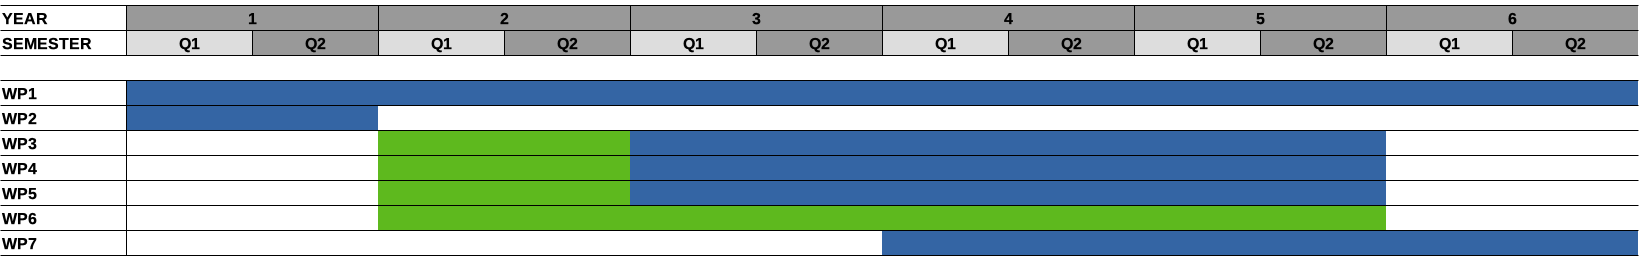
\includegraphics[width=16.5cm]{./images/workplan.png}
\caption{Research Plan Gantt Chart: {\color{RoyalBlue}$\lgblksquare \ $} Regular Research Activities; 
{\color{LimeGreen} $\lgblksquare \ $}: Activities covered by Bachelor's and Master's Thesis.} \label{fig:gantt}
\end{figure}

\subsection{Research Contacts and Collaborations}

Aside from my contacts in my current and previous research groups and centers, I gathered a significant number of research contacts and collaboration throughout my career, primarily through my research stay at MIT and research project partnerships. These contacts are important for creating project consortiums and advancing on different research fronts. Below I describe the most relevant to my research lines:


\begin{itemize}
\item Prof. Jaume Peraire, Aeronautics, and Astronautics Department at MIT: Prof. Peraire is  H.N. Slater professor of aeronautics and astronautics at MIT and former AeroAstro department head. Prof. Peraire was my host during my research stay at the Aerospace computational design laboratory.
\item Prof. Adrián Lozano Durán, Aerospace Computational Design Laboratory at MIT: The collaboration with Prof. Lozano revolves around wall modeling for Large Eddy Simulation. Prof. Lozano was an external reviewer of my Ph.D. thesis for the international mention, and we wrote a competitive research grant proposal together.
\item Dr. Francisco Ramírez. Bettair Cities S.L.: Our collaboration started in the frame of applied European projects. We have had a very productive cooperation, and we keep joining efforts to write new competitive project proposals. 
\item Prof. Darko Volkov, Worcester Polytechnic Institute: Prof. Volkov is a professor in mathematical sciences, and we met during my stay at MIT. We collaborated in developing a parallel solver for inverse problem resolution. An article was published from this collaboration. 
\item Dr. Timofey Mukha: KTH: The collaboration with Dr. Mukha is in the field of wall modeling and began back in 2018 at the ECCOMAS conference in Glasgow. Dr. Mukha implemented an open-source wall modeling library with classical formulations for OpenFoam. I plan to keep the contact to implement state-of-the-art data-driven wall models in OpenFoam and maximize the research impact.
\item Prof. Mahdi Abkar, Aarhus University: I met Prof. Abkhar at the 2022 IUTAM conference in Aahrus on deep learning applications for fluid mechanic problems. Our collaboration revolves around deep learning-based wall modeling applications for non-equilibrium flows. 
\item Prof. Mattias Liefvendahl, RISE Research Institutes of Sweden: Prof. Liefvhendahl was an external reviewer of my Ph.D. thesis for the international mention, and he is an expert in wall modeling for hydrodynamic applications.  
\item Prof. Ricardo Vinuesa, KTH: I am collaborating with Prof. Vinuesa in the field of Machine Learning-based Reduced Order Models in the context of BSC projects. 
\item Prof. Clara Garcia-Sánchez, TU Delft: The collaboration with Prof. Garcia-Sánchez stems from Urban Flow Simulation projects. At present, we are involved in a European project proposal writing regarding the use of data-driven techniques for environmental flow prediction and public health prevention.
\item Prof. Sergio Chiva Vicent, Universitat Jaume I: Our current collaboration is in the frame of a "Retos de la Sociedad" competitive project focused on 3D data-driven pollutant dispersion in urban environments. 
\item Prof. Roel Verstappen, Groningen University: Prof. Verstappen is an expert in numerical discretization methods for finite volume and subgrid modeling. Prof. Verstappen was a member of my Thesis committee.   
\item Prof. Miguel de Castro Neto, Universidade Nova Lisboa: The research relationship with Prof. de Castro started through a European H2020 project related to smart cities. Since then, we have collaborated in writing new project proposals in the field of pollutant substance dispersion modeling.
\end{itemize}


\subsection{Innovation and Technology Transfer}

I am planning to bring my fundamental and applied research activities beyond the academic sphere by promoting innovation to tackle social challenges in relevant areas such areas of energy, environment, and health prevention. These subjects are part of the 5 major missions recently identified by the European Union \href{https://ec.europa.eu/commission/presscorner/detail/en/IP_21_4747}{(see EU link)} and the United Nations \href{https://www.un.org/sustainabledevelopment}{(see UN link)} as sustainable development goals. 

To do so, I am planning to seek the support of UPC's Spin-Offs \href{https://www.upc.edu/innovacio}{(see link)} and Innovate \href{https://www.upc.edu/emprenupc}{(see link)} programs, for the creation of spin-offs and entrepreneurship activities in collaboration with industry. I will particularly encourage those activities carried out by young entrepreneurial students. On the other hand, I will manage the eventual patents and intellectual property titles resulting from patentable results and technological innovations through the UPC's Office of Patents and Licenses \href{https://www.upc.edu/innovacio/ca/oficina-patents}{(see link)}.

\subsection{Dissemination Plan} 

I plan to disseminate my research work by publishing it in high-impact journals in fluid mechanics, energy, environmental science, and machine learning. The targeted journals include Physical Review Letters, Journal of Fluid Mechanics, Journal of Computational Physics, Fluids, Physics of Fluids, Physical Review Fluids, Journal of Wind Engineering and Industrial Aerodynamics, AIAA, International Journal of Heat and Fluid Flow, Computers \& Fluids, Boundary-Layer Meteorology, Atmospheric Environment, Atmospheric Research, Journal of Turbomachinery, Progress in Energy and Combustion Science, Geoscience Data Journal, among others.

Concerning database generation for model training purposes, the created datasets will be shared according to the corresponding project data management plan. If no specific data repositories are mentioned, the research-oriented clouds of Mendeley Data, Dryad Digital Repository, Harvard Dataverse, and the Open Science Framework will be considered. The generated knowledge will also be made publicly available through open-access repositories (e.g., UPC-Commons, arXiv) and software development platforms (e.g., GitLab, GitHub).

Finally, I will also disseminate my research work by participating in national and international conferences such as WCCM-ECCOMAS, ERCOFTAC, European Fluid Mechanics Conference, IUTAM conferences, International Conference on Heat and Thermal Energy, World Conference on Earth \& Environmental Science, International Symposium on Marine Sciences, among others, seminars (e.g., Fluid Mechanics Seminars at Stanford University), and workshops (Center for Turbulence Research Summer Program at Stanford University, UPM Fluid Dynamics Group Summer Workshop in Madrid).








\newpage

\section{Teaching Plan} 

\subsection{Teaching Background} \label{sec:teach_back}

My first teaching experience started in 2001 as a Mathematics, Physics, Mechanics, Technology, and Electrical Engineering lecturer for university preparatory courses while studying for my Mechanical Engineering Master's. After this four-year period, in 2005, I moved to the industry, but I always missed being involved in teaching activities. Later, during my Ph.D. period, I had several opportunities to carry out some teaching activities related to fundamental aerodynamics in the Helicopters and Wind Energy subjects of the UPC's Aerospace Vehicle Engineering Degree and the Master in Energy, respectively. 

In September 2022, I started teaching Thermal Machines theory (Màquines Tèrmiques, 240EI021, 4.5 ECTS), a core subject of the Master in Industrial Engineering (MUEI) at the "Escola Tècnica Superior d'Enginyeria Industrial de Barcelona" (ETSEIB). Later in February 2023, I started teaching Heat Transfer theory (Termotècnia, 240171, 6 ECTS) core subject of the Industrial Engineering Bachelor Degree (GETI) at ETSEIB. Thermal Machines combine the most relevant fundamental disciplines in engineering, namely Thermodynamics, Fluid Mechanics, Heat Transfer, and Mechanics, which are essential for a deep understanding of this technological and engineering field. Specifically, thermodynamics is essential for studying machine cycles, one of the main topics of the subject in which the Carnot, Otto, Diesel, Atkinson, Stirling, Rankine, and Brayton cycles are thoroughly explained. Moreover, Fluid mechanics and aerodynamics also play an essential role, especially in the blade design of steam and gas turbines, and also in the inertial fluid effects in reciprocating engines and the fundamental role they play in engine efficiency. Heat Transfer is critical to correctly understanding the engine cooling requirements and the cooling system design, while mechanics are also fundamental to understanding the weight-balancing, mechanic frictions, and mechanical manufacturing processes. The subject also includes a topic on combustion and pollution closely related to my applied research activities on pollutant dispersion and mitigation strategies. 
I also participated in updating the subject laboratory sessions. Specifically, I helped design a new session consisting of disassembling and reassembling a working four-stroke engine. At the end of the session, the engine has to be successfully started. This session has received wide acceptance from the students compared to the previously existing sessions, which were merely descriptive and observational.  

On the other hand, the Heat Transfer subject is also closely related to my research, adding extra motivation and passion. Heat Transfer includes deriving governing PDEs for heat conduction problems and their further analytical and numerical resolution. Moreover, the convection topic allowed me to introduce fluid mechanic fundamentals to the students by deriving the Navier Stokes equations and explaining the origin and physical meaning of the Reynolds, Prandtl, and Nusselt numbers and the Model Theory. The convection topic also includes its application to Heat Exchangers. The subject also includes a numerical part where the students acquire the concepts of numerical resolution of PDEs, spatial discretization and meshing, spatial numerical schemes, temporal integration schemes, time integration stability, and boundary conditions, among others. The students practice these concepts by solving simple problems manually, and then, they learn using a real multiphysics solver. Specifically, I taught the use of Ansys Workbench software in numeric laboratory sessions. The students had to solve steady and transient heat conduction problems with different materials and boundary conditions. Taking advantage of my position as a researcher at BSC, I offered the students the optional activity of visiting the BSC facilities, including the current MareNostrum IV and the installation works of the future MareNostrum V supercomputer. The students significantly acknowledged this activity. Finally, the subject focuses on thermal radiation, solved through the radiosity method.

Given my willingness and enthusiasm to resume teaching activities, despite my full-time research position at BSC, I accepted a six-hour teaching workload per week in core subjects theory, plus the associated activities of preparing classes and teaching material, exams, and exercise corrections and answering student questions. I have made a great effort to explain complex concepts as clearly as possible, answer students' questions, and assist those who require it. This effort has been reflected in the UPC's student survey, where I scored almost the maximum qualification in the survey questions (see HAP document). The experience has been incredibly fulfilling, and I would be eager to continue teaching in the near future and beyond. 

Moreover, being in close contact with students has also benefited my research. The Heat Transfer subject allowed me to identify the most prominent students in areas related to my research. I offered them the opportunity to carry out their Bachelor Thesis at BSC on state-of-the-art topics related to data-driven models for fluid mechanics and passive-scalar transport applications. This is a win-win approach since they are offered the opportunity to complete their studies at a top-tier research center with access to world-class resources and scientific contacts while I advance on several research fronts. 

In that sense, I already co-directed a Bachelor's final thesis focused on state-of-the-art turbulent flow mode decomposition methodologies through Variational Autoencoders. The project has been highly successful and has already been submitted. On the other hand, I also advised another work related to scaling properties and dataset generation for data-driven wall modeling development. 

In November 2019, I also started advising a Ph.D. student at BSC who was working on developing data-driven wall models for complex non-equilibrium flows. The developed model can predict boundary layer laminar to turbulent transition, a breakthrough in the wall modeling field, and a paper is due to be submitted in the second half of this year.  

\subsection{Contextualization of the teaching project}

%Máster Universitario en Tecnologías Mecánicas por la Universidad Politécnica de Catalunya

Firstly, I will briefly describe the regulatory and organizational context on which this teaching project is built. In particular, I will focus on the European Higher Education Area (EHEA) and its implementation in the study plan of the Bachelor's and Master's degrees offered by the EEBE.

\subsubsection{Teaching framework in the EHEA}

In 1999 the Bologna conference initiated a process intended to transform and homogenize higher education in Europe by establishing the European Higher Education Area (EHEA). One of the main objectives was to facilitate the mobility of students and university staff (i.e., professors, researchers, and administrative staff), make higher education more inclusive and accessible, become higher education in Europe more attractive to international students, and contribute to the growth and competitiveness of the EU economy with knowledge and skills gained in Europe.

Thus, all countries participating in the EHEA agreed to:
\begin{itemize}
\item introduce a two-cycle higher education system consisting of undergraduate and
postgraduate studies (Master's and Doctorate).
\item ensure mutual recognition of qualifications and periods of learning abroad completed at other universities.
\item implement a quality assurance system to strengthen the quality and relevance of learning and teaching.
\end{itemize}

The EHEA proposes a teaching-learning model (with particular emphasis on the latter) that significantly impacts how subjects and degrees should be planned. One of the central elements of the EHEA to achieve compatibility and comparability of studies at the European level is the European Credit Transfer System (ECTS), adopted as a standard unit of measurement.
The ECTS provides a homogeneous standard to calculate the duration of courses and degrees and offers the possibility of quantifying the actual effort required by the student. Each ECTS corresponds to 25 work hours and quantifies all required activities to achieve the teaching objectives. This includes classroom (1/3) teaching theory or laboratory; teacher-led activities (1/3) such as practices and projects; The autonomous study (1/3) of the student. 

Another novel and determining aspect of the EHEA is the concept of competences. These are implemented to improve the relationship of the education system with the productive one, which is more focused on the development of capacities and practical skills. Professional competences involve a whole set of knowledge, procedures, attitudes, and traits that complement each other to enable students to correctly and efficiently react in real professional situations. The need to guarantee professional
competences require the education system to make a profound change in curricula and subjects in order to plan and evaluate them effectively.

{\bf EHEA in Spain}

The adaptation of Spanish curricula to the EHEA was established through the Ley Orgánica de Universidades (LOU) in 2007 and has been subsequently modified several times. At present, the basic structure of the academic offer of the Spanish university model is configured in three stages: Degree, Master, and Doctorate. Specifically, it establishes that the Degrees are of 240 ECTS, Masters of 60, 90, and 120 ECTS, and the Doctorate access requires at least 300 ECTS in the two previous stages. Regarding the latter, doctorates must be completed within a three-year period.

The Bachelor's and Master's degrees are classified into five areas of knowledge which specify the basic subjects that must compose a Degree in a given area, guaranteeing transversal training and reinforcing the generalist character of this cycle. Similarly,  the possibility of specializing in a particular academic project is also considered. On the other hand, it promotes teaching innovation, becoming a fundamental strategy of universities, centers, and the coordination of degrees. Finally, it reformulates the process of verification, monitoring, and accreditation of official university degrees by quality agencies, both national and regional, following the approaches developed in most EHEA countries. According to the Conference of Rectors of Spanish Universities (CRUE),  the university's primary objectives are:

\begin{itemize}
\item Provide opportunities and support inclusive and equitable education for all, based on recognizing the student's diversity of conditions and needs.
\item Strengthening social inclusion and the quality of education through the opportunities offered by digital transformation and innovative technologies.
\item Support universities and higher education institutions in their search for innovative solutions to the current challenges of our societies.
\item Protect and promote research, innovation, and transfer in all areas of knowledge, sciences, engineering, social sciences, arts, and humanities, as an essential service for social development and achieving the Knowledge Society.
\item Move towards more open and flexible teaching forms, lifelong learning, and the real and consolidated implementation of personalized and student-centered learning models that provide the necessary competencies and skills to become active, critical, and responsible citizens.
\end{itemize}

\subsubsection{The Studies at the Escola d'Enginyeria Barcelona Est (EEBE).}

The EEBE offers several Bachelor's and Master's degrees. The specific degrees of the present call are: 

Bachelor degrees:
\begin{itemize}[noitemsep]
\item Bachelor's degree in Biomedical Engineering
\item Bachelor's degree in Electrical Engineering
\item Bachelor's degree in Industrial Electronics and Automatic Control Engineering
\item Bachelor's degree in Energy Engineering
\item Bachelor's degree in Mechanical Engineering
\item Bachelor's degree in Chemical Engineering
\item Bachelor's degree in Materials Engineering.
\end{itemize}

Master's degrees:
\begin{itemize}[noitemsep]

\item Master's degree in Interdisciplinary and Innovative Engineering
\item Master's degree in Research in Mechanical Engineering
\end{itemize}

The Bachelor's degrees last four years and have a workload of 240 ECTS. Having a clear perspective of the degree's core subject syllabus is fundamental to being aware of students' backgrounds when arriving at advanced courses so that the curriculum can be appropriately designed to ensure students can follow it. The Bachelor's degrees offered at EEBE follow a common fundamental structure to ensure the knowledge of the minimum required subjects for engineering studies. Below, a list of the common core subjects is given: 

\begin{tabular}{c l c }
 {\bf Semester}       & {\bf Subject}             & {\bf ECTS}  \\ 
 \hline
 \multirow{5}{*}{1}   & Calculus  $\quad\quad\quad\quad\quad\quad\quad\quad\quad\quad\quad\quad\quad\quad\quad\quad\quad\quad\quad\quad\quad\quad\quad\quad\quad$                                    & 6 \\ 
                      & Chemistry                                     & 6 \\
                      & Graphic Expression                            & 6 \\
                      & Informatics                                   & 6 \\
                      & Physics I: Fundamentals of Mechanics          & 6 \\                     
\hline
 \multirow{5}{*}{2}   & Algebra and Multivariable Calculus            & 6 \\  
                      & Environmental Technologies and Sustainability & 6 \\
                      & Materials Science and Technology              & 6 \\
                      & Numerical Calculus. Differential Equations    & 6 \\   
                      & Physics II: Fundamentals of Electromagnetism  & 6 \\ 
\hline
 \multirow{5}{*}{3}   & Electrical Systems                            & 6 \\  
                      & Fluid Mechanics                               & 6 \\
                      & Mechanical Systems                            & 6 \\
                      & Statistics                                    & 6 \\   
                      & Industrial Control and Automation             & 6 \\  

\hline
 \multirow{3}{*}{4}   & Business                                      & 6 \\  
                      & Electronic Systems                            & 6 \\  
                      & Thermodynamics and Heat Transfer              & 6 \\   
\hline
\end{tabular}


Then, each Bachelor's degree has its particular core and optional subjects related to the degree's field of knowledge. 

Regarding the Master's degree, the student's origin may be diverse, and thus, being more difficult to assume a common background. In this regard, the Master's access requirements recommend that the applicants have a university-level qualification of a scientific-technical nature, i.e., a bachelor's or pre-EHEA degree in engineering or sciences. On the other hand, the academic committee of the Master's degree may consider admitting applicants who have completed qualifications other than those recommended. When such applicants are admitted, the academic committee will specify the bridging courses that must be completed.  

\subsection{Subjects of the present call and profile adequacy}

This section is intended to review the syllabus of the subjects related to the present call to objectively analyze my adequacy for the position. The subjects are distributed in two tables corresponding first to Bachelor's degree and then to Master's degree subjects:

\begin{tabular}{l l l }
{\bf Bachelor's degree subject}       &  {\bf Topic}  & $\ $                                                 \\ 
\hline
Fluid Mechanics     & 1             &  Fundamentals concepts. Fluid Properties.            \\ 
(820013)            & 2             &  Hydrostatics.                                       \\
$\ $                & 3             &  Basic concepts for flow analysis.                   \\
$\ $                & 4             &  Basic integral equations in fluid mechanics I       \\
$\ $                & 5             &  Basic integral equations in fluid mechanics II      \\   
$\ $                & 6             &  Pipe flow.                                          \\
$\ $                & 7             &  Free surface flows.                                 \\
\hline
Thermodynamics and Heat Transfer  $\quad\quad$ & 1    &  Introduction to Thermodynamics.   \\ 
(820020)            & 2             &  First law of Thermodynamics.                        \\
$\ $                & 3             &  Second Law of Thermodynamics.                       \\
$\ $                & 4             &  Conductive Heat Transfer.                           \\
$\ $                & 5             &  Convective Heat Transfer.                           \\   
$\ $                & 6             &  Radiative Heat Transfer.                            \\
\hline
Fluid Engineering   & 1             &  Fundamental Equations in differential form.         \\ 
(820425)            & 2             &  Dimensionality and similarity modeling.             \\
$\ $                & 3             &  Compressible flow.                                  \\
$\ $                & 4             &  Fluid systems.                                      \\
$\ $                & 5             &  Lift and drag. External flow.                       \\   
$\ $                & 6             &  Turbo and volumetric machinery.                     \\
\hline
 Thermal Engineering  & 1           &  Thermal Generation and Solar energy use.            \\ 
(820427)              & 2           &  Heat Exchangers.                                    \\
$\ $                  & 3           &  Gas power cycles. Compressors,                      \\
$\ $                  &   $\ $      &  Turbomachinery and reciprocating engines.           \\
$\ $                  & 4           &  Steam power cycles. Steam turbines,                 \\
$\ $                  &   $\ $      &  cogeneration.                                       \\
$\ $                  & 5           &  Cooling systems and heat pumps.                     \\  
$\ $                  & 6           &  Energy efficiency. Heat recovery. Insulation.       \\ 
\hline
Hydraulic and Thermal Machinery & 1 &  Hydraulic Turbomachinery Overview.                  \\ 
(820463)              & 2           &  Rotodynamic pumps.                                  \\
$\ $                  & 3           &  Fans.                                               \\
$\ $                  &   $\ $      &  Hydraulic Turbines.                                 \\
$\ $                  & 4           &  Similarity Laws and Characteristic curves.          \\
$\ $                  & 5           &  Wind Turbines.                                      \\ 
$\ $                  & 6           &  Reciprocating Compressors.                          \\
\hline
Computational Fluid Mechanics and Heat Transfer & 1 &  Introduction.  \\ 
(820464)              & 2           &  Mathematical models.                                \\
$\ $                  & 3           &  Dynamics behavior analysis.                         \\
$\ $                  &   $\ $      &  Feedback systems.                                   \\
$\ $                  & 4           &  Introduction to CFD.                                \\
$\ $                  & 5           &  Discretization techniques.                          \\ 
$\ $                  & 6           &  Coupled and non-linear systems.                     \\
\hline
\end{tabular}

\begin{tabular}{l l l }
{\bf Master's degree subject}       &  {\bf Topic}  & $\ $                                                 \\ 
\hline
Computational fluid Mechanics  & 1  &  Numerical Methods.                                  \\ 
(205609 - 205609)   & 2             &  Navier-Stokes flow solver.                          \\
$\ $                & 3             &  High Performance Computing.                         \\
$\ $                & 4             &  Computational Flow Physics.                         \\     
\hline
Systems Modeling  $\quad\quad\quad\quad\quad\quad\quad\quad\quad\quad\quad\quad\quad\ \ $ & 1  &  Mathematical modeling of systems.                    \\ 
(295104 - 295II014) & 2             &  Classical theory of partial differential  $\quad\quad\quad\ $          \\
$\ $                  &   $\ $      &  equations.                                          \\
$\ $                & 3             &  General theory of partial differential              \\
$\ $                  &   $\ $      &  equations.                                          \\
$\ $                & 4             &  Multiphysics and multiscale modeling.               \\

\hline
\end{tabular}

As described in the teaching background section (see sec. \ref{sec:teach_back}), I have experience as a Thermal Machines theory lecturer and collaborated in laboratory sessions. I also have experience in Heat Transfer theory and numerical sessions. Below, a table with the subject's syllabus is given for comparison with the EEBE's Fluid Mechanics Department subjects.

\begin{tabular}{l l l }
{\bf Subject}       &  {\bf Topic}  & $\ $                                                 \\  
\hline
Thermal Machines $\quad\quad\quad\quad\quad\quad\quad\quad\quad\quad\quad\quad\quad\ \ $ & 1 &  Energy transformations  $\quad\quad\quad\ $          \\
(295104 - 295II014)                 &   2  &  Classification, applications, and theoretical      \\
$\ $                &   $\ $        &  Thermodynamic cycles of Thermal Machines.  \\
$\ $                & 3             &  4-stroke reciprocating engines              \\
$\ $                & 4             &  2-stroke reciprocating engines                                          \\
$\ $                & 5             &  Engine performance and environmental impact   \\ 
$\ $                & $\ $          &  of reciprocating engine.  \\
$\ $                & 6             &  Wankel Engine.  \\
$\ $                & 7             &  Gas turbines.  \\
$\ $                & 8             &  Rocket engines.  \\
$\ $                & 9             &  Fuels.  \\
$\ $                & 10            &  Steam turbine power plants.  \\
$\ $                & 11            &  Stirling engine.  \\
\hline
Heat Transfer       & 1             &  Introduction. Energy balances.              \\
(240171 - 240171)   & 2             &  1D steady conduction.                           \\
$\ $                & 3             &  Numerical Methods (steady and transient).  \\
$\ $                & 4             &  Convection. Model Theory and              \\
$\ $                & $\ $          &  Heat Exchangers.              \\
$\ $                & 5             &  Thermal Radiation                               \\
\hline
\end{tabular}

By comparing the syllabus of the call subjects with my previous experience, it becomes clear that my profile is suitable for the "Thermodynamics and Heat Transfer" and "Thermal Engineering" subjects. Moreover, I could rapidly adapt to the "Hydraulic and Thermal Machinery" subject. On the other hand, most of the other department's subjects perfectly fit with my research background and lines. In that sense, my profile is also suited for "Fluid Mechanics", "Fluid Engineering", "Computational Fluid Mechanics and Heat Transfer", and "Computational fluid Mechanics" subjects. In conclusion, I could start teaching seven of the Fluid Mechanics department subjects out of eight from the beginning.     

Some adaptations may be needed. However, I want to remark that since September 2022, I have prepared and taught two core subjects of the Industrial Engineering Bachelor's and Master's degrees despite having another full-time research position at BSC, which shows my ability to adapt to new teaching challenges. 

\subsection{Training Plan Innovation}

The training innovation plan focuses on creating new Master's subjects with the aim of teaching relevant knowledge and skills in some innovative areas that, in my opinion, after studying the teaching guide, are not sufficiently covered.

In recent years, Machine Learning and derived methodologies such as Deep Learning have become effective tools for solving an extraordinary variety of problems, including fluid mechanics and other relevant engineering problems. In that sense, all engineers should have a minimum level of knowledge of these methodologies, the same way it is assumed that minimal knowledge of statistics, numerical methods, or even programming is required. By inspecting the Bachelor's degrees syllabus, there is an optional subject on "artificial intelligence applied to engineering" (820055). However, among the methodologies proposed in the subject, the most widely used deep learning techniques, namely, neural networks, are omitted. In that sense, I would like to propose the creation of an optional subject on advanced deep-learning methods applied to fluid mechanics and heat transfer problems. This subject would provide the students with the fundamentals of neural networks, including Multilayer Perceptrons (MLP) and Convolutional Neural Networks (CNN), backpropagation, optimization, activation, and loss functions.

After providing the neural network fundamentals, the subject would be focused on using MLPs to obtain data-driven solutions of physical models mathematically described by Partial Differential Equations by introducing the concept of physics-informed, a methodology intended to enforce physical laws in the data-driven models. The methodology of Raissi et al. \cite{RAI17}, which first introduced the physics-informed concept, would be followed. In the second step, the application of CNNs to fast predict the lift and drag coefficients of aerodynamic airfoils will be used. 

The required datasets to successfully carry out the teaching plan can be obtained from open-source repositories such as AirRANS \href{https://airfrans.readthedocs.io/en/latest/index.html}{(see link)}. At the same time, free online Google Colab services with Jupyter notebooks and GPU training hardware could be used for neural network implementation and training. In that sense, predefined Colab templates could be provided to students to focus on the relevant coding parts and avoid the need to spend time on less-important parts such as dataset loader creation. 

Given that most students may be unfamiliar with the theoretical background, this subject should be at least 6 ECTS credits long. The subject would combine theoretical sessions, especially in the first phase, and then laboratory programming sessions to implement the models. The evaluation would be done through exams for the theoretical part and final individual works on the neural network implementation. 

A more extended subject, including other architectures such as Recurrent Neural Networks, could also be introduced in the Interdisciplinary \& Innovative Engineering and Research in Mechanical Engineering Masters. In the particular case of the Interdisciplinary \& Innovative Engineering Masters, it already includes Data Analysis \& Pattern Recognition (295102-295II012) and Computer Vision (295106-295II022) as core subjects. This previous knowledge could be leveraged to go further in the engineering application aspect. In that sense, the extensive dataset in urban flow and pollutant dispersion generated during my research projects can be used to create a specific subject on advanced deep learning-based urban flow and pollutant dispersion modeling. A publication explaining the dataset generation process and the physical and numerical modeling techniques will be submitted in the final quarter of this year. This publication will also make publicly available the datasets, which will be uploaded in the open-source repository \href{https://www.pangaea.de/}{https://www.pangaea.de/} according to the project's data management plan, so they will be available for students to download. 

Given that students of the Interdisciplinary \& Innovative Engineering Masters can be assumed with previous knowledge of neural networks, this subject could be 4.5 ECTS credits long. Similarly, the subject would combine theoretical sessions on more advanced architectures, especially in the first phase, and then laboratory programming sessions to implement the models. The evaluation would also be done through exams for the theoretical part and final individual works on the neural network implementation. 

\subsection{Teaching methodology Innovation}

Traditionally in University courses, master classes have been the methodology used, where the student is a mere receiver of Professors' knowledge. In this methodology, the student easily forgets the concepts after the exam. Other methodologies foster meaningful learning, where the student learns by linking the new concepts with their
previous knowledge, facilitating the concept's internalization to further apply them to many other situations. A key aspect for engineering students is that in their professional careers, they will have to face situations different from those typical cases explained in lectures. 

I want to introduce new methodologies based on meaningful knowledge in my future teaching activity. One example of this is problem-based learning performed in small groups. The concepts are provided previously to the students by notes made by the Professor, provided bibliography, or even a virtual class recorded by the Professor that students have to read/listen to on their own. This is called Flipped Classroom (FC) methodology. The FC is a pedagogical model that transfers part of the learning process outside the classroom (i.e., students watch recorded classes on their own) and uses class time, together with the Professor's experience, to facilitate and enhance other processes of acquisition and practice of knowledge, facilitating the student to develop skills for critical assessment. Moreover, students work on their interpersonal relationships and teamwork capability, which will be a key competence in most of their professional careers as engineers. Besides, in that context, I will encourage them to make presentations in class on the outcome of the problem resolution.
This methodology has been successfully used in Thermal Machines (Màquines Tèrmiques) course I started in September 2022. Students were encouraged to develop innovative power plants based on thermal systems by considering renewable heat sources, alternative fuels, congeneration processes, etc. Fundamentals on thermal heat plants were only partially taught in class, forcing the student to do some research on their own. Then, discussions on the project's progress were encouraged in class. Final works were developed in groups of a maximum of five students and presented in class to their student colleagues.

On the other hand, programming is a fundamental competence that any engineer should have, and students should be able at least to solve relatively simple engineering problems by coding. Since informatics is a first-year core subject, it can be assumed that students can do so. In that sense, I will promote creating small programs to solve physical and engineering problems whenever possible. Although the UPC provides some licenses for popular programming tools like Matlab, I support open-source libraries and codes to ensure that students can apply the acquired abilities after finishing their studies regardless of their professional or personal circumstances. In that sense, I will promote using open-source programming languages and libraries, such as Python and Julia, to carry out the proposed exercises and projects. 

I want also to promote the use of open-source software tools in class. In the Thermal Machines subject, it was mandatory to size the thermal power plant through the open-source Steam System Modeler Tool (SSTM) of the U.S. Energy Department \href{https://www4.eere.energy.gov/manufacturing/tech_deployment/amo_steam_tool/overview}{(see link)}. Moreover, the use of Lotus Engine Simulator was also encouraged to simulate the particular case of a two-stroke reciprocating engine exhaust system \href{https://www.lotusengineering.com/engineering-software/}{(see link)}. 

In the present Heat Transfer course, I used the Ansys Workbench software to carry out a numerical exercise concerning the resolution of steady and transient heat conduction problems. The choice of the simulation software was agreed with all the department faculty. Nevertheless, as previously commented, my point of view is to promote using open-source codes whenever possible and switch to tools such as OpenFOAM. On the other hand, using OpenFOAM for other physics, such as computational fluid dynamics, is also within my pedagogical objectives for Fluid Mechanics-related subjects, such as Computational Fluid Mechanics and Heat Transfer, to resolve applied problems. 

According to my experience in the Thermal Engine laboratory sessions, the sessions that generated more interest among students involved real working devices. Some of the sessions were focused on the mere observation of engine parts or inoperative engines and barely motivated students. In that sense, I contributed to designing a new session where students had to disassemble and reassemble an operative four-stroke Otto engine. The final step of the session consisted in successfully starting the engine. The devices were simple, low-cost cost engines that still had the most relevant components of an Otto engine and allowed the students to effectively understand the engine's working principles. The participants were highly motivated by this session and acknowledged its inclusion in the subject's laboratory sessions program. This experience encouraged me to promote laboratory sessions featuring fully operational devices whenever possible. 

%ASSIGNATURES ONLINE

%Due to my experience in the Thermal Engine laboratory sessions, I concluded that the sessions %that generated more interest among students by far were those in which real working devices were %involved. Some of the sessions were focused on the mere observation of engine parts or %inoperative engines and barely motivated students. In that sense, I contributed to designing a %new session in which students had to disassemble and reassemble an operative four-stroke Otto %engine. The final step of the session consisted in successfully starting the engine. The devices %were simple, low-cost cost engines that still had the most relevant components of an Otto engine %and allowed one to effectively understand the engine's working principles. The students were %extremely motivated by this session, and they acknowledged their participation. This experience %encouraged me to promote laboratory sessions featuring fully operational devices to draw % students' attention and motivation. In that sense, it would be interesting to create synergies %with other departments to leverage existing unused resources, such as the gas turbine testing %bench available in the aeronautics department.  

In order to further improve my abilities as a university lecturer, I also plan to subscribe to UPC's "Institut de Ciències de l'Educació" (ICE) courses. Some of the courses listed below, which are currently offered by the ICE are highly motivating for me:

\begin{itemize}[noitemsep]
\item Subject syllabus design based on challenges.
\item Teaching / Postgraduate in STEAM.
\item Teaching support services and ATENEA's subject portal improvement. 
\item Introduction to the statistics software R.
\item Non-violent communication for conflict prevention.
\item Mapathon: How to analyze the working environment in a collaborative manner.
\end{itemize}

\subsection{Bachelor's, Master's, and Ph.D. Thesis Planning} 

Bachelor's and Master's final thesis are an excellent opportunity to advance in relatively small fronts of the planned research objectives. The objective feasibility must be carefully evaluated, and the requirements must be adjusted depending on the student's background and capabilities. On the other hand, teaching at the university offers the possibility to identify the most prominent students and give them the opportunity to work in state-of-art subjects. The most capable and motivated ones would be encouraged to enroll in a doctoral program.
The works will be planned in advance to train the student in deep learning before starting the thesis work. This strategy has been successfully applied to the works I co-directed or advised so far. Below, some Bachelor's, Master's, and Ph.D. topic proposals aligned with the research objectives described in section \ref{sec:res-obj} are given. Moreover, these topics are also based on my personal opinion that deep learning methods should be widely taught and used for tackling engineering problems:

{\bf Bachelor's Final Thesis.} 

\begin{itemize}[noitemsep]
\item 2D Graph Neural Networks for Spatial Physical Problems in 2D.
\item 2D Reduced-order models for turbulent flow prediction through Variational Autoencoder's latent space evolution forecast.
\end{itemize}

{\bf Master's Final Thesis.}

\begin{itemize}[noitemsep]
\item Graph Neural Network for 3D unstructured mesh data processing. Wall Modeling Applications.
\item Graph Neural Network-based Variational Autoencoders for flow modal decomposition and reconstruction in 3D unstructured meshes.
\item Graph Neural Network for large 3D unstructured mesh data. Applications to WMLES simulation data processing.
\item Data-driven data assimilation techniques for initial condition generation.
\item Data-driven techniques for experimental measurement quality enhancement.  
\item Data-driven techniques for variable reconstruction from experimental measurement data. 
\item Active flow-control technology analysis  through wall-modeled Large Eddy Simulations.
\end{itemize}
%afegir per a motors algo amb el paper que vaig trobar

{\bf Ph.D. Thesis.}

\begin{itemize}[noitemsep]
\item Contextual Wall Models Through Graph Neural Networks. Application to complex flow aerodynamics. OpenFOAM implementation.
\item High-fidelity fast urban flow prediction with thermal and inner layer obstacle effects.
\item Fast time-predictive tools for environmental flows through data-driven reduced order models. 
\end{itemize}

\subsection{Personal vision on the studies}

My perspective is motivated as a former engineering student and current Professor on the Industrial Engineering Bachelor and Master's degrees at UPC. To this end, I divide the courses into general groups depending on their functionality.

\begin{itemize}
\item Fundamental courses: must teach the necessary knowledge for the student to understand the whole degree. They set the foundations. Examples are physics, calculus, chemistry, etc.
\item Core courses: must teach the basic knowledge needed to understand future courses and set the basis of basic knowledge a student should have. They are the trunk. Examples are:
Fluid Mechanics, Thermodynamics, Heat Transfer, etc.
\item Specialized courses: where more advanced knowledge is being taught. They are based on core and fundamental courses to expand the students' knowledge to specialized areas. Examples are Fluid Engineering, Numerical Fluid Mechanics, Heat Transfer, etc.
\item Free elective courses: these courses give students first contact with a topic of interest related to their studies. It is a great opportunity for them to get acquainted with the research done by professors and complement their knowledge on a particular topic. In that sense, I would be eager to contribute to creating new innovative subjects in applied machine learning for engineering problems solving. 
\end{itemize}

Aside from the aforementioned technical knowledge, in my opinion, students should also acquire other important skills to successfully develop their professional careers, such as:

\begin{itemize}
\item developing transversal competences that will be useful to them in further studies or their work.
\item understanding and synthesizing knowledge and being able to produce good-quality reports. 
\item programming basic codes to solve engineering problems.
\item producing good quality presentations that are understandable to their peers, etc.
\end{itemize}

All these abilities can be practiced while learning the core skills needed for an engineer.

\subsection{Equality and Inclusion}

As a member of a social minority, I am especially aware of the difficulties that collectives such as women or LGTBI community members may face in daily life, also in their studies or workplaces. For this reason, I was a founder member of the equality team at the BSC's CASE department to help promote equality within the group and assist people that may need it. In that sense, I would be eager to pursue this activity at the UPC. 

The UPC's equality plan \href{https://igualtat.upc.edu/ca/shared/third-upc-gender-equality-plan.pdf}{(see link)} establishes that special attention will be dedicated to equity, diversity \& inclusion by promoting the balance in the recruitment, admission, and retention of researchers. In this regard, I am willing to participate in existing initiatives such as the "Aquí STEAM UPC" program, which focuses on attracting female talent to technology and engineering studies to break stereotypes and gender roles and encourage primary and high school students from underrepresented and/or economically disadvantaged groups, and students in general, to overcome barriers and pursue STEM careers. 


\newpage

\begin{thebibliography}{9}

\bibitem{CAL19}
J. Calafell, F.X. Trias, O. Lehmkuhl and A. Oliva. A time-average filtering technique to improve the efficiency of two-layer wall models for large eddy simulation in complex geometries. {\it Computers \& Fluids}, Vol. 188 pp. 49-59 (2019) \href{https://doi.org/10.1016/j.compfluid.2019.03.026}{https://doi.org/10.1016/j.compfluid.2019.03.026} 

\bibitem{ALJ18}
D.E. Aljure, J. Calafell, A. Baez, A. Oliva. Flow over a realistic car model: Wall modeled large eddy simulations assessment and unsteady effects. {\it Journal of Wind Engineering and Industrial Aerodynamics}, Vol. 174, pp. 225-240 (2018) \href{https://doi.org/10.1016/j.jweia.2017.12.027}{https://doi.org/10.1016/j.jweia.2017.12.027}

\bibitem{KUT17}
J. Kutz. Deep learning in fluid dynamics. {\it Journal of Fluid Mechanics} Vol. 814, pp. 1-4, (2017) \href{https://doi.org/10.1017/jfm.2016.803}{https://doi.org/10.1017/jfm.2016.803}

\bibitem{TOP17}
Y. Toparlar, B. Blocken, B. Maiheu and G.J.F. van Heijst. A review on the CFD analysis of urban microclimate. {\it Renewable and Sustainable Energy Reviews}, Vol. 80, pp. 1613-1640, (2017) \href{https://doi.org/10.1016/j.rser.2017.05.248}{https://doi.org/10.1016/j.rser.2017.05.248}


\bibitem{MOK21}
S. Mokhtar, M. Beveridge, Y. Cao, and I. Drori. Pedestrian Wind Factor Estimation in Complex Urban Environments. {\it  Proceedings of The 13th Asian Conference on Machine Learning}. Vol. 157, pp. 486-501, (2021) \href{https://proceedings.mlr.press/v157/mokhtar21a/mokhtar21a.pdf}{https://proceedings.mlr.press/v157/mokhtar21a/mokhtar21a.pdf}

\bibitem{HOI22}
H. Høiness, K. Gjerde, L. Oggiano, K. Teigen, and M. Ruocco. Positional Encoding Augmented GAN for the Assessment of Wind Flow for Pedestrian Comfort in Urban Areas. {\it arXiv} (2022) \href{https://arxiv.org/pdf/2112.08447.pdf}{https://arxiv.org/pdf/2112.08447.pdf} 


\bibitem{SLO14} J. Slotnick, A. Khodadoust, J. Alonso, D. Darmofal, W. Gropp, E. Lurie, and D. Mavriplis, CFD vision 2030 study: A path to revolutionary computational aerosciences, NASA Langley Research Center Report No. NASA/CR-2014-218178, 2014 (unpublished), available at \href{http://ntrs.nasa.gov/archive/nasa/casi.ntrs.nasa.gov/20140003093.pdf}{http://ntrs.nasa.gov/archive/nasa/casi.ntrs.nasa.gov/20140003093.pdf}

\bibitem{BOS18} S. Bose, Sanjeeb and G.I.Park, Wall-Modeled Large-Eddy Simulation for Complex Turbulent Flows. Annu. Rev. Fluid Mech. 50,pp 535-561 (2018) \href{https://doi.org/10.1146/annurev-fluid-122316-045241}{https://doi.org/10.1146/annurev-fluid-122316-045241}

\bibitem{VAR23} A. Vardot, X.I.A. Yang, and M. Abkar. Survey of machine-learning wall models for large-eddy simulation. {\it Phys. Rev. Fluids}, Vol. 8(6), pp. 064603 (2023) \href{https://link.aps.org/doi/10.1103/PhysRevFluids.8.064603} {https://link.aps.org/doi/10.1103/PhysRevFluids.8.064603}

\bibitem{ZHO20} J. Zhou, G. Cui, S. Hu, Z. Zhang, C. Yang, Z. Liu, L. Wang, C. Li and M. Sun.
Graph neural networks: A review of methods and applications. {\it AI Open}, Vol. 1, pp. 57-81, (2022). \href{https://doi.org/10.1016/j.aiopen.2021.01.001}{https://doi.org/10.1016/j.aiopen.2021.01.001}

\bibitem{GAO22} H. Gao and S. Ji. Graph U-Nets. {\it IEEE Trans Pattern Anal Mach Intell.} Vol. 44(9), pp. 4948-4960. (2022) \href{https://ieeexplore.ieee.org/document/9432709}{doi: 10.1109/TPAMI.2021.3081010}

\bibitem{GUA23} L. Guastoni, J. Rabault, P. Schlatter, H. Azizpour, and R. Vinuesa. Deep reinforcement learning for turbulent drag reduction in channel flows. {\it The European Physical Journal}, Vol. 46(4), pp. 27, (2023) \href{https://pubmed.ncbi.nlm.nih.gov/37039923/}{DOI: 10.1140/epje/s10189-023-00285-8}

\bibitem{RAB19} J. Rabault, M. Kuchta, A. Jensen, U. Réglade and N. Cerardi. Artificial neural networks trained through deep reinforcement learning discover control strategies for active flow control. {\it Journal of Fluid Mechanics}. Vol. 865, pp. 281-302 (2019) \href{https://www.cambridge.org/core/journals/journal-of-fluid-mechanics/article/abs/artificial-neural-networks-trained-through-deep-reinforcement-learning-discover-control-strategies-for-active-flow-control/D5B80D809DFFD73760989A07F5E11039}{DOI: 10.1017/jfm.2019.62}

\bibitem{VIA21} J.M. Viana Parente Lopes, J.M.L.M. Palma, and A. Silva Lopes. Modelling the flow within forests: the canopy-related terms in the Reynolds-averaged formulation. {\it Journal of Fluid Mechanics}. Vol. 910, A7, (2021). \href{https://doi.org/10.1017/jfm.2020.927}{https://doi.org/10.1017/jfm.2020.927}

\bibitem{LIM09} H.C. Lim, T.G. Thomas, and I.P. Castro. Flow around a cube in a turbulent boundary layer: LES and experiment. {\it Journal of Wind Engineering and Industrial Aerodynamics}. Vol. 97, pp. 96-109, (2009). \href{https://doi.org/10.1016/j.jweia.2009.01.001}{https://doi.org/10.1016/j.jweia.2009.01.001}

\bibitem{EIX22} B. Eiximeno, A. Miró, J.C. Cajas, O. Lehmkuhl, and I. Rodríguez. On the wake dynamics of an oscillating cylinder via proper orthogonal decomposition. {\it Fluids}, Vol. 7(9), p. 1-23 (2022). \href{https://doi.org/10.3390/fluids7090292}{https://doi.org/10.3390/fluids7090292} 

\bibitem{EIV22} H. Eivazi, S. LeClainche, S. Hoyas, and R. Vinuesa. Towards extraction of orthogonal and parsimonious non-linear modes from turbulent flows. {\it Expert Systems with Applications}, Vol. 202, pp. 117038, (2022) \href{https://doi.org/10.1016/j.eswa.2022.117038}{https://doi.org/10.1016/j.eswa.2022.117038}.

\bibitem{LEE21} S. Lee and D. You. Analysis of a convolutional neural network for predicting unsteady volume wake flow fields. {\it Physics of Fluids} Vol. 33(3), pp. 35152 (2021) \href{https://doi.org/10.1063/5.0042768}{https://doi.org/10.1063/5.0042768}

\bibitem{LOP21} M. Lopez-Martin, S. Le Clainche, and B. Carro. Model-free short-term fluid dynamics estimator with a deep 3D-convolutional neural network. {\it Expert Systems with Applications}, Vol. 177, pp. 114924, (2021) \href{https://doi.org/10.1016/j.eswa.2021.114924}{https://doi.org/10.1016/j.eswa.2021.114924}

\bibitem{ABA22} R. Abadía-Heredia, M. López-Martín, B. Carro, J.I. Arribas, J. Pérez, and S. Le Clainche. A predictive hybrid reduced order model based on proper orthogonal decomposition combined with deep learning architectures. {\it Expert Systems with Applications}, Vol. 187, pp. 115910, (2022) \href{https://doi.org/10.1016/j.eswa.2021.115910}{https://doi.org/10.1016/j.eswa.2021.115910}

\bibitem{TAV81} S. Tavoularis and S. Corrsin. Experiments in nearly homogenous turbulent shear flow with a uniform mean temperature gradient. Part 1. {\it Journal of Fluid Mechanics}, Vol. 104, pp. 311 - 347, (1981) \href{https://doi.org/10.1017/S0022112081002930}{https://doi.org/10.1017/S0022112081002930}

\bibitem{WEA20} J. Weatheritt, Y. Zhao, R.D. Sandberg, S. Mizukami, K. Tanimoto. Data-driven scalar-flux model development with application to jet in cross flow. {\it International Journal of Heat and Mass Transfer} Vol. 147, pp. 118931, (2020) \href{https://doi.org/10.1016/j.ijheatmasstransfer.2019.118931}{https://doi.org/10.1016/j.ijheatmasstransfer.2019.118931}

\bibitem{MIL18} Pedro M. Milani, Julia Ling, Gonzalo Saez-Mischlich, Julien Bodart, John K. Eaton-A Machine Learning Approach for Determining the Turbulent Diffusivity in Film Cooling Flows 
{\it Journal of Turbomachinery}, Vol. 140(2), pp. 021006, (2018) \href{https://doi.org/10.1115/1.4038275}{https://doi.org/10.1115/1.4038275}

\bibitem{ALM22} V.A. de Almeida, H.F. de Campos Velho, G.B. França, and N.F.F Ebecken. Neural networks for data assimilation of surface and upper-air data in Rio de Janeiro. {\it Geosci. Model Dev. Discuss.} [preprint], (2022) \href{https://doi.org/10.5194/gmd-2022-50}{https://doi.org/10.5194/gmd-2022-50} 

\bibitem{ARC21} R. Arcucci, J. Zhu,S. Hu, and Y.K Guo. Deep Data Assimilation: Integrating Deep Learning with Data Assimilation. {\it Appl. Sci.}, Vol. 11(3), pp. 1114, (2021) \href{https://doi.org/10.3390/app11031114}{https://doi.org/10.3390/app11031114}

\bibitem{HAS23} G. Hasanuzzaman, H. Eivazi, S. Merbold, C. Egbers, and R. Vinuesa. Enhancement of PIV measurements via physics-informed neural networks. {\it Measurement Science and Technology}, Vol. 34 pp. 044002. (2023) \href{https://iopscience.iop.org/article/10.1088/1361-6501/aca9eb}{DOI 10.1088/1361-6501/aca9eb}

%\bibitem{VIN23} R. Vinuesa, S.L. Brunton, and B.J. McKeon. The transformative potential of machine learning for experiments in fluid mechanics. {\it arXiv} (2023) \href{https://doi.org/10.48550/arXiv.2303.15832}{https://doi.org/10.48550/arXiv.2303.15832}

\bibitem{MON22} V. Mons, O. Marquet, B. Leclaire, P. Cornic, and F. Champagnat. Dense velocity, pressure and Eulerian acceleration fields from single-instant scattered velocities through Navier–Stokes-based data assimilation. {\it Measurement Science and Technology}, Vol. 33 pp. 124004. (2022) \href{https://iopscience.iop.org/article/10.1088/1361-6501/aca9eb}{https://iopscience.iop.org/article/10.1088/1361-6501/ac8dac}

\bibitem{RAI17} R. Maziar and P. Perdikaris, and G.E. and Karniadakis. Physics Informed Deep Learning (Part II): Data-driven Discovery of Nonlinear Partial Differential Equations. {\it arXiv} (2017) \href{https://doi.org/10.48550/arXiv.1711.10561}{https://doi.org/10.48550/arXiv.1711.10561}

%\bibitem{THI21} I. Thiam, B. Khady Thiam, and I. Faye. Numerical Simulation of Ocean Currents with Hermite IFinite Elements. {\it International Journal of Applied Mathematics and Theoretical Physics}, Vol. 7(4), pp. 112-125, (2021) \href{https://www.sciencepublishinggroup.com/journal/paperinfo?journalid=322&doi=10.11648/j.ijamtp.20210704.14}{doi: 10.11648/j.ijamtp.20210704.14}

\bibitem{VOL19}
D. Volkov and J. Calafell. A stochastic approach to reconstruction of faults in elastic half-space. {\it Inverse Problems \& Imaging}, Vol. 13(3) pp. 479-511 (2019) \href{http://dx.doi.org/10.3934/ipi.2019024}{http://dx.doi.org/10.3934/ipi.2019024} 


\bibitem{JOF23} L. Jofre, A. Abdellatif, and G. Oyarzun. RHEA: an open-source Reproducible Hybrid-
architecture flow solver Engineered for Academia. {\it Journal of Open Source Software} Vol. 8(81), pp. 4637, (2023). \href{https://doi.org/10.21105/joss.04637}{https://doi.org/10.21105/joss.04637}

\bibitem{HOU09} G. Houzeaux, M. Vázquez, R. Aubry, and J.M. Cela. A massively parallel fractional step solver for incompressible flows. {\it Journal of Computational Physics}. Vol. 228(17), pp. 6316-6332, (2009) \href{https://doi.org/10.1016/j.jcp.2009.05.019}{https://doi.org/10.1016/j.jcp.2009.05.019}









\end{thebibliography}

\end{document}




\subsubsection{Teaching framework in the EHEA}

The joint declaration of the European education ministers, meeting at the Ministerial Conference in Bologna in June 1999, initiated a process of transformation and homogenization of higher education in Europe. The changes that this process implies are multiple and deep.

The Bologna process established the European Higher Education Area (EHEA) to facilitate the
mobility of students and university staff (i.e., professors, researchers, and administrative staff), make higher education more inclusive and accessible, become higher education in Europe more attractive to foreign students, and contribute to the growth and competitiveness of the EU economy with knowledge and skills gained in Europe.

Thus, all countries participating in the EHEA agreed to:
\begin{itemize}
\item introduce a two-cycle higher education system, consisting of undergraduate and
postgraduate studies (Master's and Doctorate).
\item ensure mutual recognition of qualifications and periods of learning abroad completed at
other universities.
\item implement a quality assurance system to strengthen the quality and relevance of learning
and teaching.
\end{itemize}

The time horizon for the implementation of the EHEA was before 2010. In the successive
Ministerial Conferences held on the EHEA, the state of development of the plan is continuously evaluated and there is a majority agreement that recognizes that the level of compliance is satisfactory, and that great progress has been made in the aspects of mobility of teachers and students, of homogeneity in the recognition of the studies and aptitudes of the students as well as in the requirements to access higher studies or the labor market. Also noteworthy is the degree of internationalization of universities that has been achieved and the increase in cooperation in teaching and research.

The EHEA proposes a teaching-learning model (with special emphasis on the latter) that has a
very important impact on the way in which subjects and degrees should be planned. One of the
central elements of the EHEA to achieve compatibility and comparability of studies at European
level is the European Credit Transfer System (ECTS), adopted as a common unit of measurement.
The ECTS, in addition to providing a homogeneous standard to calculate the duration of courses
and degrees, offers the possibility of quantifying the real effort required by the student. Each ECTS corresponds to 25 hours of work and quantifies all the activities required to achieve the teaching objectives. This includes classroom (1/3) teaching theory or laboratory; teacher-led activities (1/3) such as practices and projects; The autonomous study (1/3) of the student. 

Another novel and determining aspect of the EHEA is the concept of competences. These are implemented to improve the relationship of the education system with the productive one, which is
more focused on the development of capacities and practical skills. Professional competences involve a whole set of knowledge, procedures, attitudes, and traits that complement each other so
that the individual must "know," "know how to do," and "know how to be" to act effectively in
professional situations. It is an integrative concept because it contemplates both skills and
attitudes so that it goes beyond the technical components. Competences involve knowing what needs to be done and being able to deal with it in a real situation. The need to guarantee professional
competences requires the education system to make a profound change in curricula and subjects
in order to plan and evaluate them effectively.

{\bf EHEA in Spain}

The adaptation of Spanish curricula to the EHEA was established through the Ley Orgánica de Universidades (LOU) of 2007. Subsequently, the Real Decreto 1393/2007, of 29 October, specified the new structuring of official university education and degrees, reorienting, with due regulatory support, the aforementioned process of convergence of our university education with the principles of the EHEA.

The organization of official university education has been subject to up to ten modifications of different entities, the most recent being carried out by Real Decreto 822/2021, of September 28. The basic structure of the academic offer of the Spanish university model is configured in three stages: Degree, Master, and Doctorate. In that sense, it consolidates that the Degrees are of 240 ECTS1, Masters of 60, 90, and 120 ECTS, and the Doctorate to which access exceeds 300 ECTS in the two previous stages.

This legislation introduces a significant modification by changing the assignment of the Bachelor's and Master's degrees of the five branches of knowledge to the so-called fields of knowledge. These areas of knowledge specify the basic subjects that must compose a Degree of the area, guaranteeing transversal training and reinforcing the generalist character of this cycle. The fields of knowledge largely follow the structure of the International Standard Classification of Education. Similarly, this Real Decreto introduces the possibility of adopting specific forms of articulation of the curriculum in official education and, therefore, of singularizing its academic project. On the other hand, it promotes teaching innovation so that it becomes a fundamental strategy of universities, centers, and coordination of degrees. Finally, it reformulates the process of verification, monitoring, and accreditation of official university degrees by quality agencies, both national and regional, following the approaches developed in most EHEA countries.

To conclude the section on how the EES has been implemented in Spain, it should be noted that the Conference of Rectors of Spanish Universities (CRUE) has recently assumed the following specific commitments:

\begin{itemize}
\item Provide opportunities and support inclusive and equitable education for all, based on the recognition of the diversity of conditions and needs in which students find themselves.
\item Strengthening social inclusion and the quality of education through the opportunities offered by digital transformation and innovative technologies.
\item Support universities and higher education institutions in their search for innovative solutions to the current challenges of our societies.
\item Protect and promote research, innovation, and transfer in all areas of knowledge, sciences, engineering, social sciences, arts, and humanities, as an essential service for social development and for the achievement of the Knowledge Society.
\item Move towards more open and flexible teaching forms, towards lifelong learning, and towards the real and consolidated implementation of personalized and student-centered learning models that provide the necessary competencies and skills to become active, critical, and responsible citizens.
\end{itemize}